\documentclass[10pt,twocolumn]{article}
\usepackage[margin=0.75in]{geometry}
\usepackage{amsmath,graphicx,booktabs,xcolor}\usepackage[expansion=false]{microtype}
\usepackage[hidelinks]{hyperref}
\usepackage[font=small,labelfont=bf]{caption}
\graphicspath{{../docs/img/}}
% Generated by  python -m adamas.paper  from the ADAMAS package. Do not edit by hand.
\newcommand{\BFOMratio}{48{,}976}
\newcommand{\KappaRatio}{14.7}
\newcommand{\MeasuredOverSi}{89}
\newcommand{\BestBV}{3659}
\newcommand{\LossSi}{209.5}
\newcommand{\LossSiC}{29.7}
\newcommand{\LossGaN}{20.6}
\newcommand{\LossDiamond}{3.8}
\newcommand{\LossDiamondMeasured}{89}
\newcommand{\GateTimeUs}{25}
\newcommand{\FcohPublished}{0.998}
\newcommand{\qForSixtySeven}{0.75}
\newcommand{\qForEightyTwo}{0.87}
\newcommand{\ReadoutContrast}{45}
\newcommand{\Polarization}{82}
\newcommand{\LambdaFast}{4.03}
\newcommand{\LambdaMs}{3.56}
\newcommand{\LambdaTenMs}{2.64}
\newcommand{\RSADistance}{57}
\newcommand{\RSAQubitsM}{78}
\newcommand{\RSADieMm}{5.7}
\newcommand{\RSAYears}{6.0}
\newcommand{\RSAYearsFast}{1.0}
\newcommand{\RSADaysSC}{4}
\newcommand{\DiaCells}{323}
\newcommand{\NumRefs}{541}
\newcommand{\NumVerified}{500}
\newcommand{\NumFigures}{52}
\newcommand{\UncPowerPten}{2.5}
\newcommand{\UncPowerPfifty}{3.8}
\newcommand{\UncPowerPninety}{5.5}
\newcommand{\UncQPten}{1.2}
\newcommand{\UncQPfifty}{3.6}
\newcommand{\UncQPninety}{15.5}
\newcommand{\ValChecks}{19}
\newcommand{\ValPass}{18}
\newcommand{\ThrCSSBias}{0.63}
\newcommand{\ThrXZZXBias}{1.59}
\newcommand{\ThrDepol}{0.95}
\newcommand{\NativeGain}{12}
\newcommand{\RSADistanceCSSBiased}{129}
\newcommand{\RSAQubitsMCSSBiased}{399}
\newcommand{\RSAYearsCSSBiased}{13.6}
\newcommand{\RSADistanceXZZX}{53}
\newcommand{\RSAQubitsMXZZX}{67}
\newcommand{\RSAYearsXZZX}{5.6}
\newcommand{\SobolMobility}{0.42}
\newcommand{\SobolField}{0.42}
\newcommand{\SobolReadout}{0.96}
\newcommand{\XZZXDepolQubitsM}{142}
\newcommand{\CSSDepolQubitsM}{165}
\newcommand{\BreakevenStdMs}{100}
\newcommand{\BreakevenXZZXMs}{1000}

\newcommand{\repo}{\href{https://github.com/Normansrule/adamas-diamond-framework}{github.com/Normansrule/adamas-diamond-framework}}
\newcommand{\site}{\href{https://normansrule.github.io/adamas-diamond-framework/}{normansrule.github.io/adamas-diamond-framework}}

\title{\textbf{ADAMAS: an open, tested framework for diamond electronics\\and room-temperature nitrogen-vacancy quantum processors}}
\author{Aleksander Norman\\\small California State University, Dominguez Hills\\\small\repo}
\date{Preprint, generated from the repository}

\begin{document}
\twocolumn[\maketitle\begin{abstract}
Diamond combines the largest breakdown field and thermal conductivity of any practical semiconductor with a defect, the nitrogen-vacancy (NV) center, whose electron spin is a qubit at room temperature. ADAMAS is an open framework that follows one path from wafer to quantum processor with executable, cited models: \NumRefs{} references (\NumVerified{} verified against Crossref), \NumFigures{} regenerable figures, a process design kit with a placed 4-bit processor, circuit-level quantum error correction, and hands-on experiments from US\$100 upward. Three results stand out. (i) Measured hydrogen-terminated diamond transistors already beat silicon's one-dimensional limit by $\sim$\MeasuredOverSi$\times$, and in an 800\,V traction inverter an ideal diamond switch loses \LossDiamond\,W against \LossSiC\,W for silicon carbide. (ii) Evaluated with the published parameters of the 2013 room-temperature entangled pair, coherence alone would permit a Bell fidelity of \FcohPublished; the measured 0.67 corresponds to a charge-state preparation probability of \qForSixtySeven, identifying preparation, not coherence, as the bottleneck. (iii) Circuit-level simulations with idle errors during millisecond readout show that surface-code scaling survives only while readout stays below about a tenth of the nuclear-memory coherence time, that a bias-tailored XZZX code extends this about tenfold, and that a factoring-scale machine fits on a \RSADieMm\,mm die but runs for years. Every number in this paper is generated from the package.
\end{abstract}\vspace{1em}]

\section{Introduction}
Silicon's dominance rests on process maturity, not material merit. For power conversion, high-temperature electronics, and room-temperature quantum technology, diamond's figures of merit are extreme: its Baliga figure of merit for power switches is \BFOMratio$\times$ silicon's and its thermal conductivity \KappaRatio$\times$ \cite{baliga1982,wei1993}. Its obstacles are equally concrete: boron acceptors sit 0.37\,eV deep, so under 1\% ionize at room temperature \cite{lagrange1998}; single-crystal wafers only recently reached 3 inches \cite{e6orbray2026}; and logic has been p-channel only until the first n-channel MOSFET in 2024 \cite{liao2024}.

ADAMAS treats these facts as inputs to models that can be run, tested, and falsified. The contribution is not a new device but a connected, reproducible chain: materials $\rightarrow$ process $\rightarrow$ circuits $\rightarrow$ qubits $\rightarrow$ error correction $\rightarrow$ machine size $\rightarrow$ experiments, with each link checked against published data or an independent tool (ngspice, Icarus Verilog, Yosys, KLayout, Stim, PyMatching).

\section{Power devices and converters}
\begin{figure}[t]\centering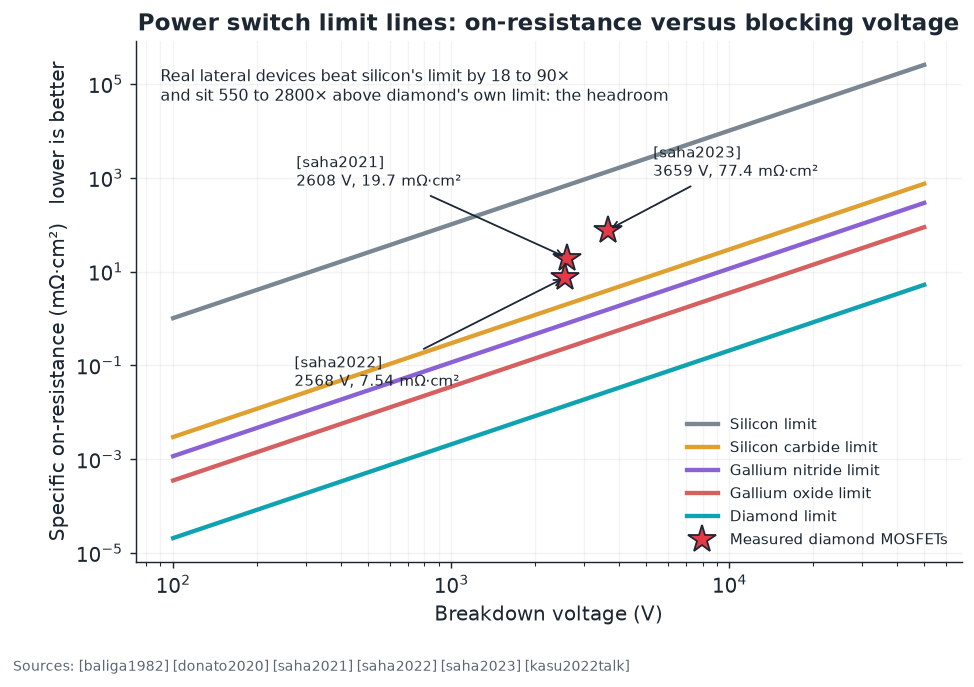
\includegraphics[width=\columnwidth]{fig03_ron_vs_bv.png}
\caption{One-dimensional on-resistance limits and measured hydrogen-terminated diamond MOSFETs \cite{saha2021,saha2022,saha2023}. Real devices sit above diamond's own limit but below silicon's.}\label{fig:ron}\end{figure}
The unipolar limit $R_{on,sp}=4BV^2/(\varepsilon\mu E_c^3)$ \cite{baliga1982} places ideal diamond far below every other material (Fig.~\ref{fig:ron}). Measured lateral hole-gas transistors reach \BestBV\,V \cite{saha2023} and, at 2568\,V, 7.54\,m$\Omega$\,cm$^2$ \cite{saha2022}, about \MeasuredOverSi$\times$ better than silicon's limit. For an area-optimized hard-switched leg, conduction and switching losses equalize and the loss is $P=2IV\sqrt{fR_{on,sp}C_{oss,sp}/2}$ \cite{erickson2020}. Table~\ref{tab:inv} shows the result for an 800\,V, 300\,A, 20\,kHz traction inverter; bulk-doped diamond additionally improves with temperature as boron ionizes \cite{pernot2010}.
\begin{table}[h]\centering\small\begin{tabular}{lr}\toprule Switch (1.2\,kV class) & Loss per switch (W)\\\midrule
Silicon, ideal & \LossSi\\ Silicon carbide, ideal & \LossSiC\\ Gallium nitride, ideal & \LossGaN\\ Diamond, ideal & \LossDiamond\\ Diamond, 2022 device scaled & \LossDiamondMeasured\\\bottomrule\end{tabular}
\caption{Area-optimized switch loss in an 800\,V, 300\,A, 20\,kHz inverter leg (first order: no gate charge or reverse recovery).}\label{tab:inv}\end{table}

\section{Process, design kit, and a placed processor}
\begin{figure*}[t]\centering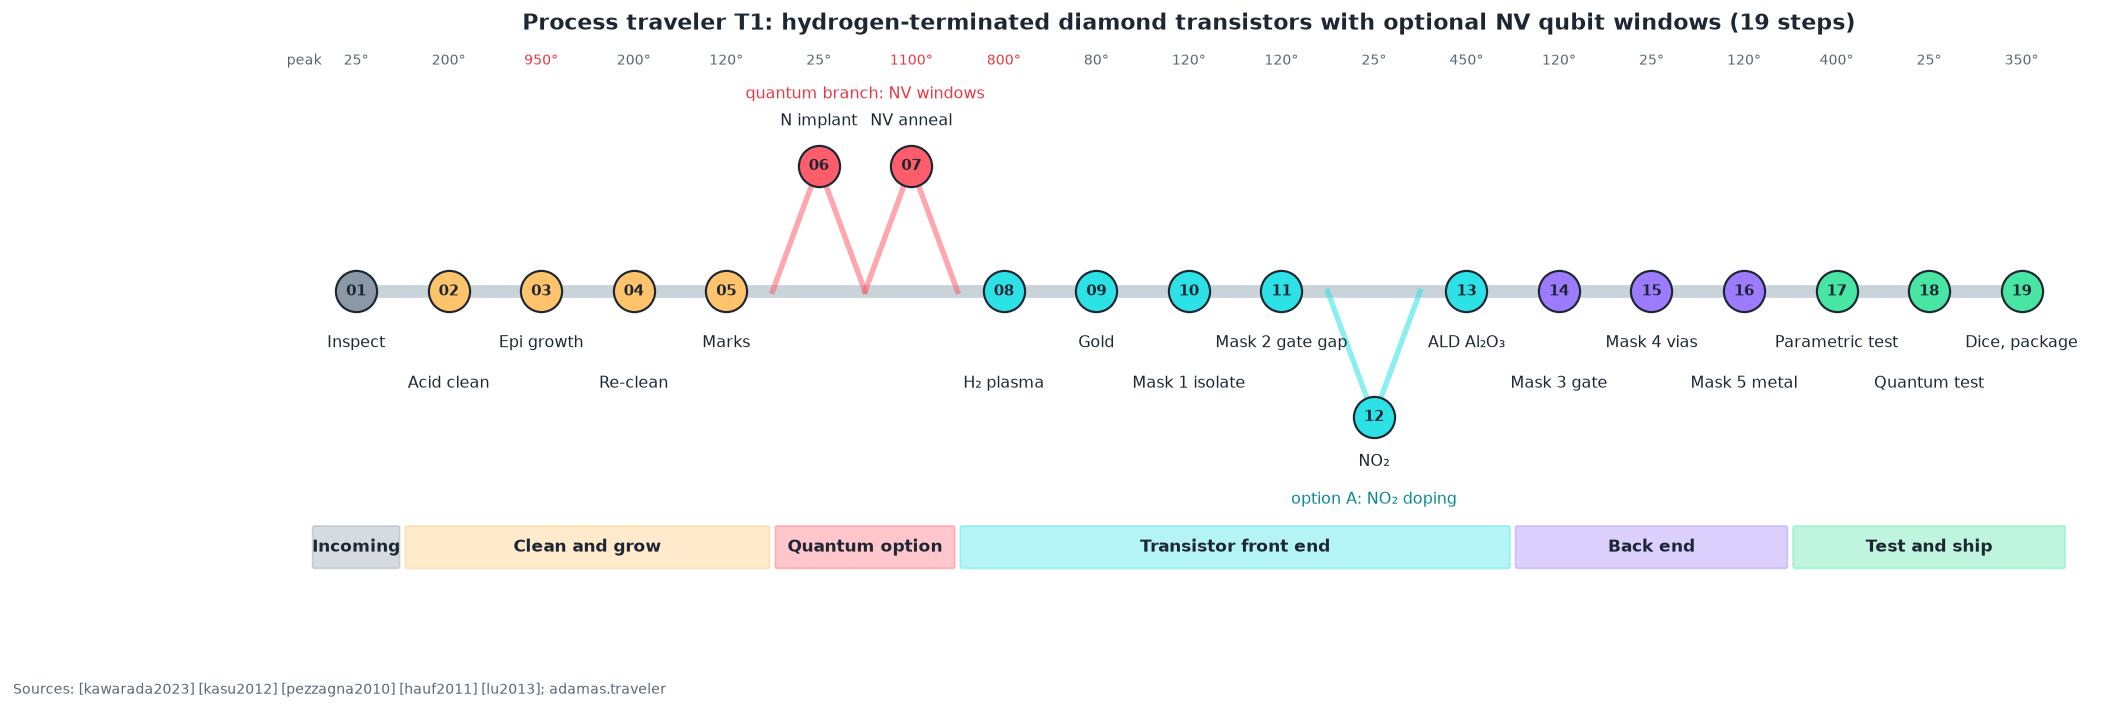
\includegraphics[width=\textwidth]{fig41_process_flow.png}
\caption{Process traveler T1: 19 steps from a bare plate to a tested chip, with a quantum branch (NV implant and anneal) and an NO$_2$ doping option. Heat is spent before the first metal.}\label{fig:flow}\end{figure*}
The hydrogen-terminated flow (Fig.~\ref{fig:flow}) creates the channel by surface transfer doping \cite{maier2000}, protects it with gold immediately, isolates devices with one oxygen-plasma step, and stabilizes the hole gas with atomic-layer-deposited Al$_2$O$_3$ at $\le$150\,$^\circ$C (with NO$_2$) or $\sim$450\,$^\circ$C (for 400\,$^\circ$C operation) \cite{kasu2012,kawarada2014,kawarada2023}. Its thermal budget forces growth and the NV anneal (up to 1100\,$^\circ$C \cite{pezzagna2010}) ahead of all metal. The traveler gives parameters with sources, pass criteria, safety, and failure modes for each step, and an interactive run log. On this process, the design kit PDK-0 supplies layers, rules, a GDS monitor die, standard cells, LEF abstracts, and a timed Liberty file; the DIA-4 processor synthesizes to \DiaCells{} cells and places in about 1\,mm$^2$ with pads. An emulator matches its Verilog cycle for cycle on random programs.

\section{The two-qubit bottleneck}
\begin{figure}[t]\centering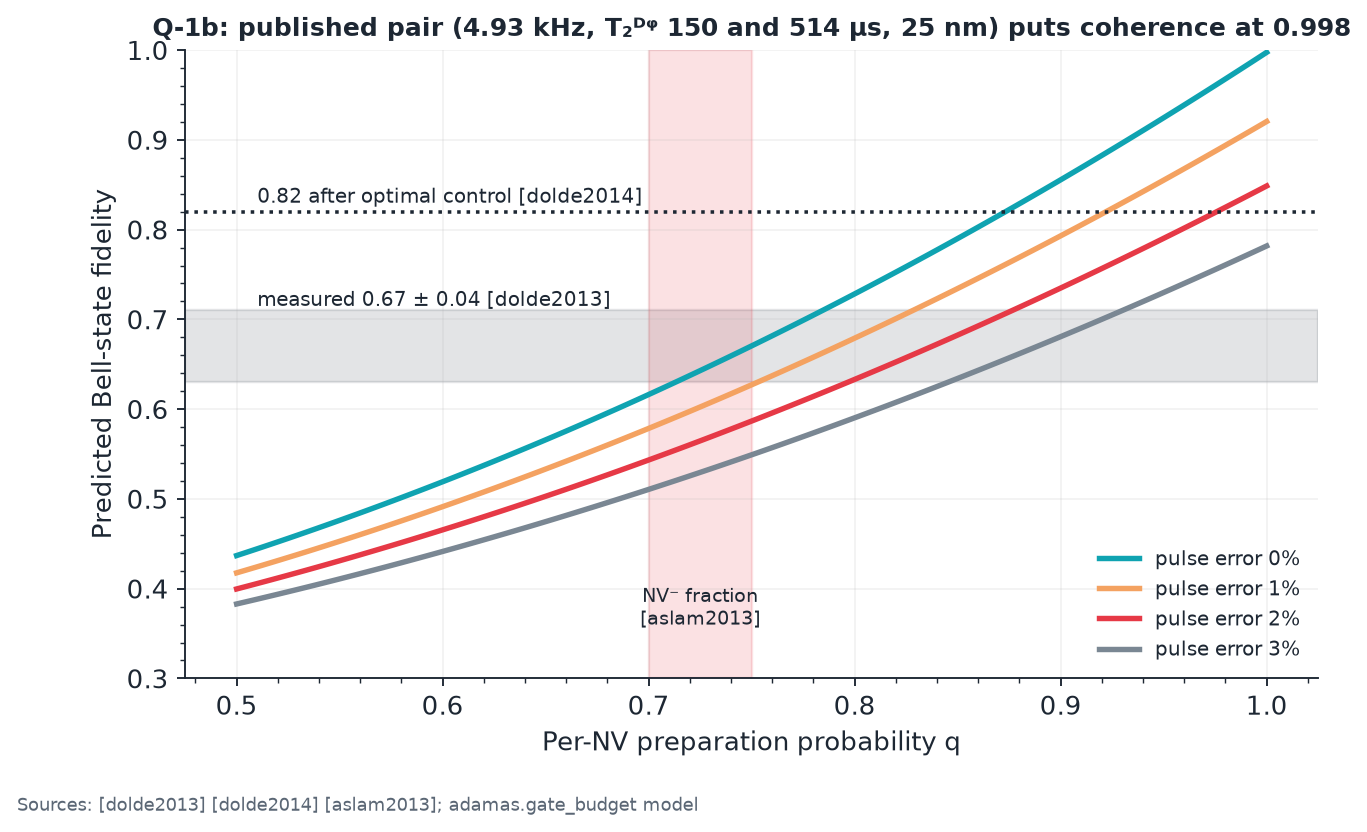
\includegraphics[width=\columnwidth]{fig36_published_gate_check.png}
\caption{Echoed NV--NV gate budget evaluated with the published pair \cite{dolde2013}: fidelity versus charge-state preparation probability. Coherence limits fidelity to \FcohPublished.}\label{fig:gate}\end{figure}
With the published pair's parameters, 25\,nm spacing, 4.93\,kHz single-quantum coupling (a \GateTimeUs\,$\mu$s double-quantum gate), and echo times of 150 and 514\,$\mu$s \cite{dolde2013}, the coherence-limited Bell fidelity is \FcohPublished. The measured 0.67 corresponds to a preparation probability $q=\qForSixtySeven$ and the later 0.82 \cite{dolde2014} to $q=\qForEightyTwo$ (Fig.~\ref{fig:gate}). Both match the NV$^-$ fraction under green light \cite{aslam2013}. A five-level rate model with measured rates \cite{tetienne2012} gives a readout contrast of \ReadoutContrast\% in a 300\,ns window and \Polarization\% spin polarization; charge-state verification before the gate is therefore the highest-leverage experimental change.

\section{Error correction with slow readout}
\begin{figure}[t]\centering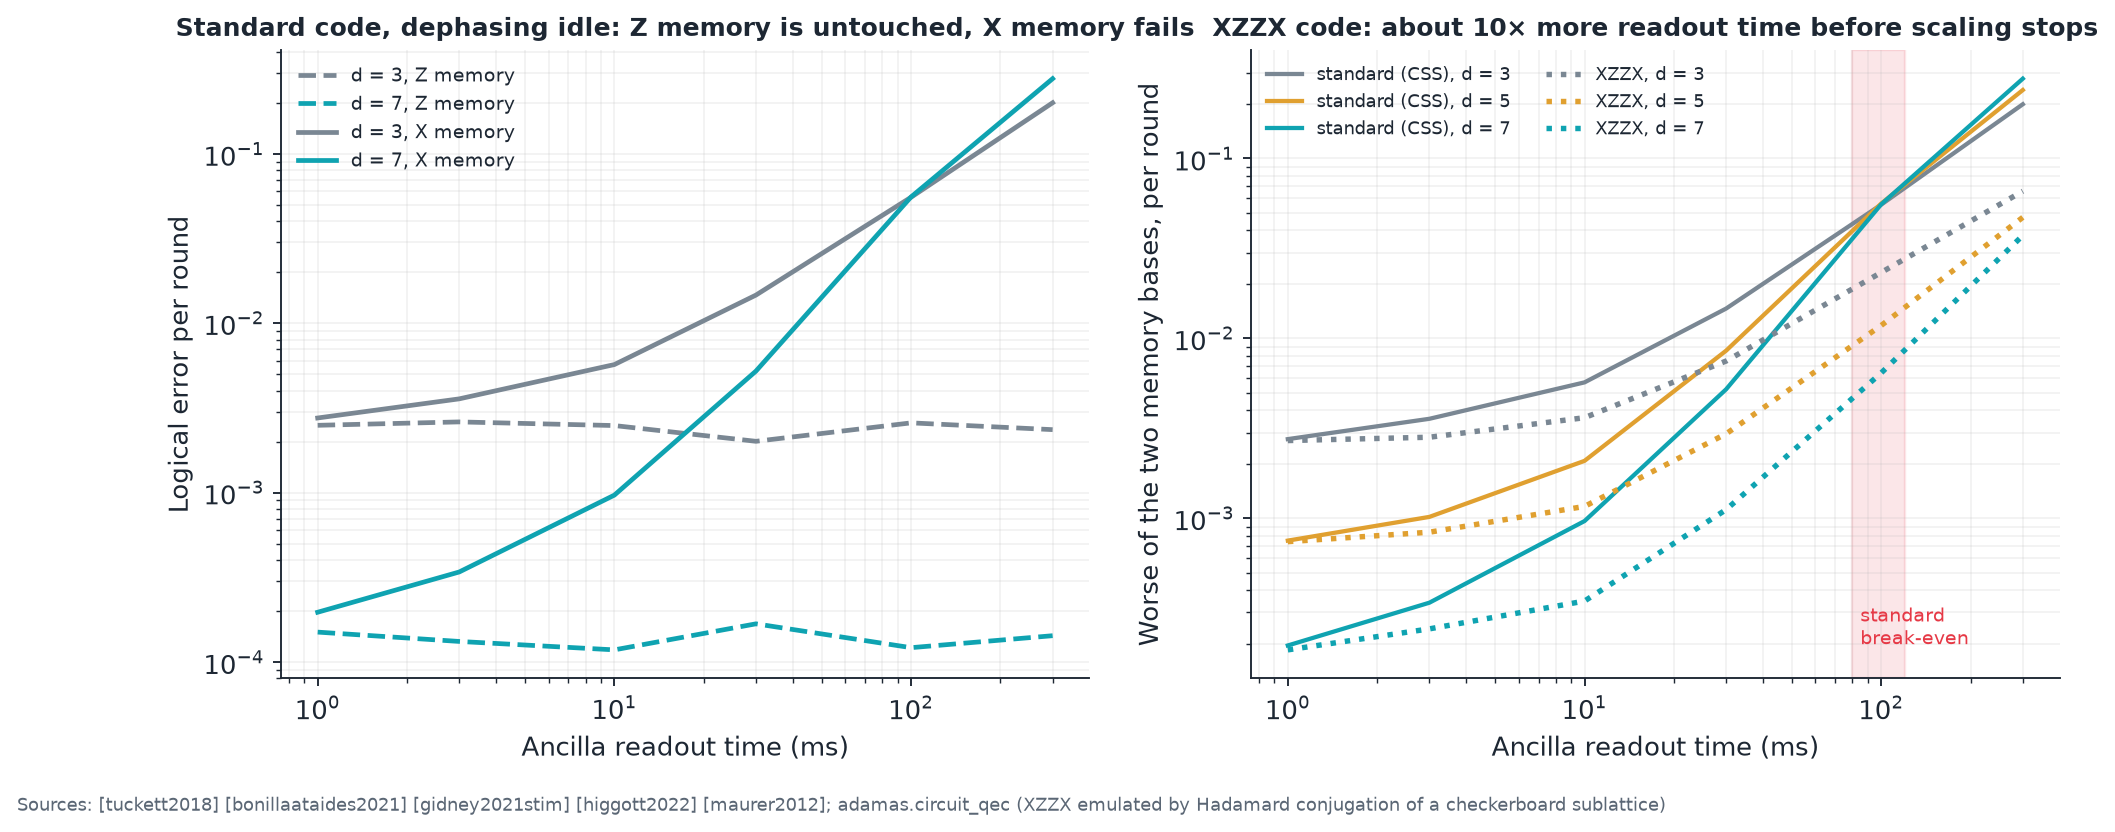
\includegraphics[width=\columnwidth]{fig40_biased_noise_xzzx.png}
\caption{Circuit-level surface code with dephasing idle errors during readout. Left: standard code, Z and X memories. Right: worse basis for standard and XZZX codes.}\label{fig:xzzx}\end{figure}
NV readout takes about a millisecond \cite{neumann2010science,hopper2018}, during which data qubits held in nuclear spins idle. Circuit-level simulations with Stim and PyMatching \cite{gidney2021stim,higgott2022} (0.3\% link, 1\% readout, 0.2\% preparation errors) validate a threshold near 1.2\% for uniform noise and give an error-suppression factor $\Lambda=\LambdaFast$ at 0.1\,ms readout, \LambdaMs{} at 1\,ms, and \LambdaTenMs{} at 10\,ms for a 1\,s memory. Distance 7 stops beating distance 3 near \BreakevenStdMs\,ms. Nuclear memories mostly dephase; the standard code wastes this bias because its X memory fails first, while an XZZX code \cite{tuckett2018,bonillaataides2021}, emulated by Hadamard conjugation of a checkerboard sublattice, pushes break-even to about \BreakevenXZZXMs\,ms (Fig.~\ref{fig:xzzx}). Building the XZZX syndrome circuit natively (CZ and XCX gates on one sublattice, so hook errors are included) and giving the gates biased noise confirms this at the gate level: at bias $\eta=100$ the standard code's threshold falls from \ThrDepol\% to \ThrCSSBias\% while the XZZX threshold rises to \ThrXZZXBias\%, and for an NV cell at 1\,ms readout the distance-7 XZZX memory is \NativeGain$\times$ better than the standard one (Fig.~\ref{fig:native}).
\begin{figure}[t]\centering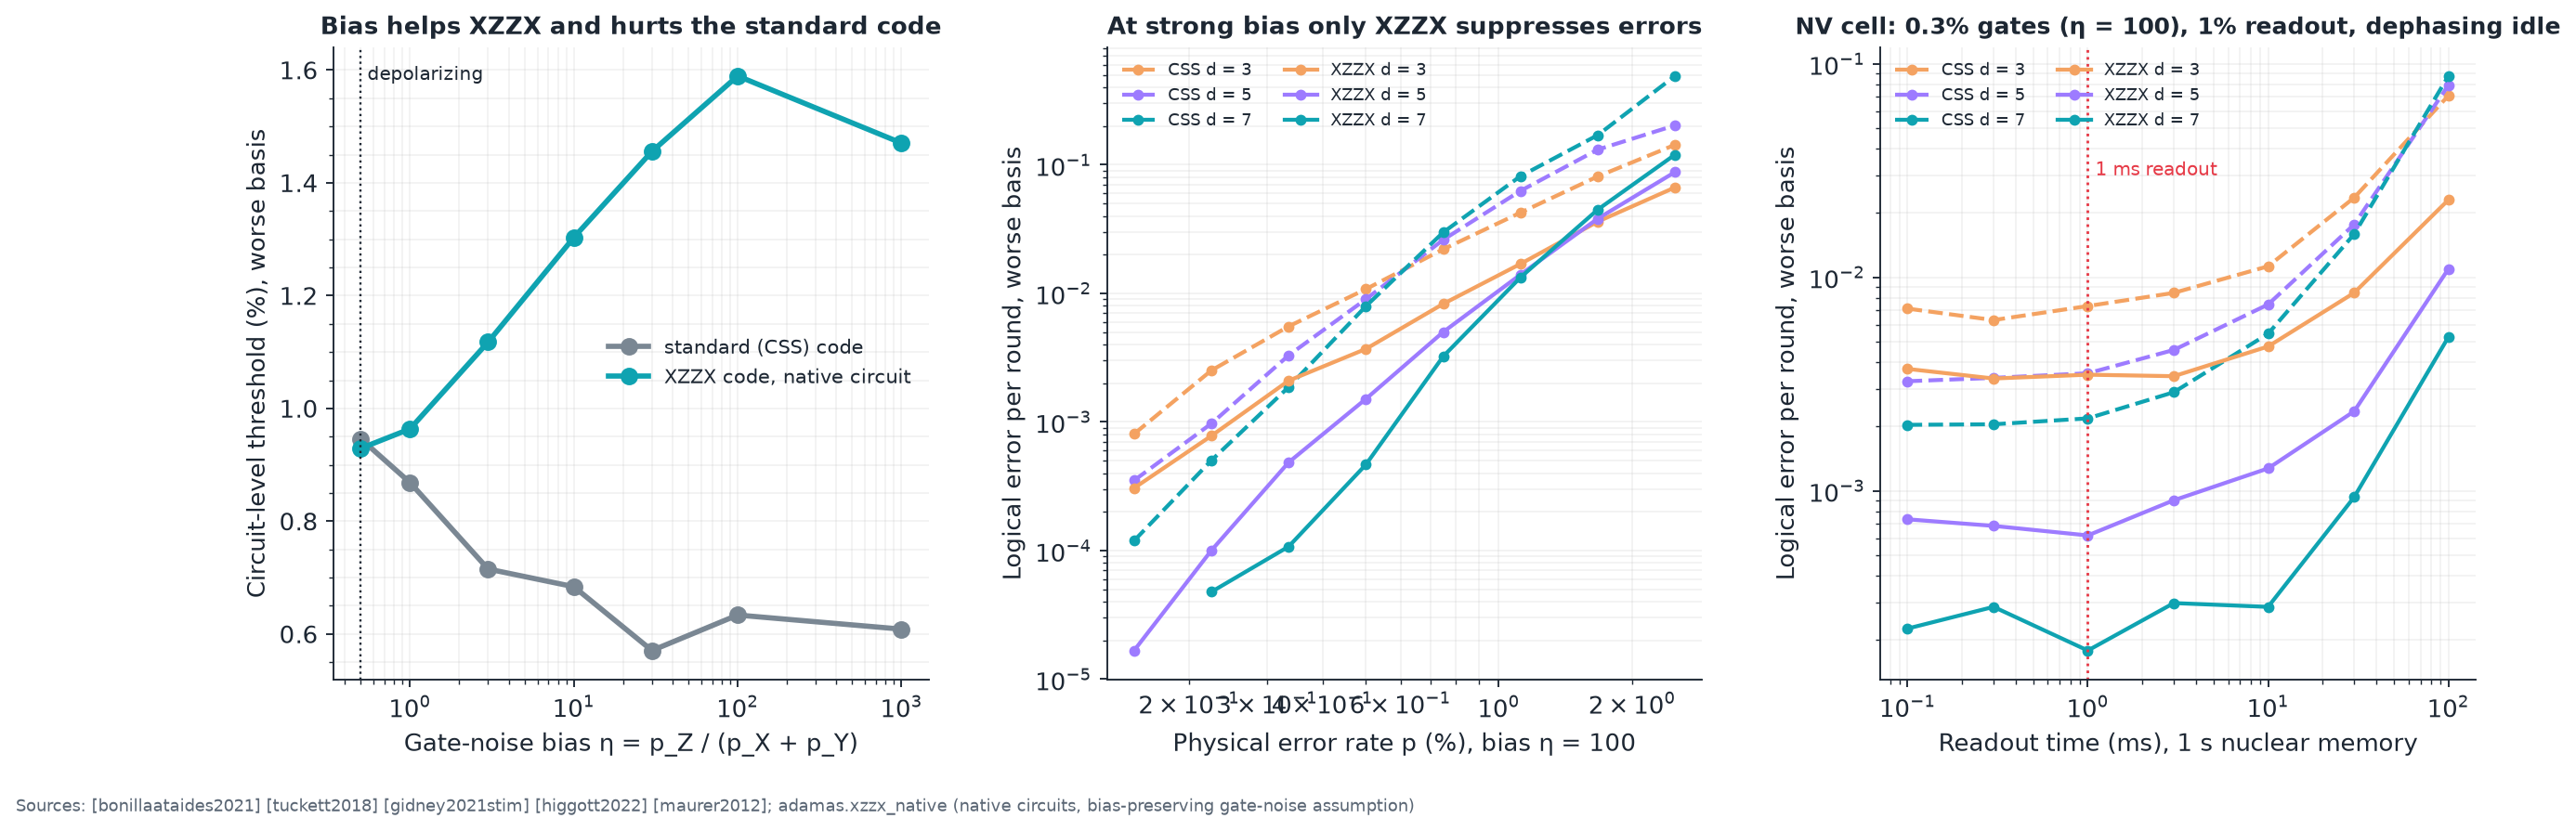
\includegraphics[width=\columnwidth]{fig50_xzzx_native.png}
\caption{Native XZZX circuits with biased gate noise: thresholds versus bias, logical error at $\eta=100$, and the NV readout scenario.}\label{fig:native}\end{figure}

\section{How big, how slow}
\begin{figure}[t]\centering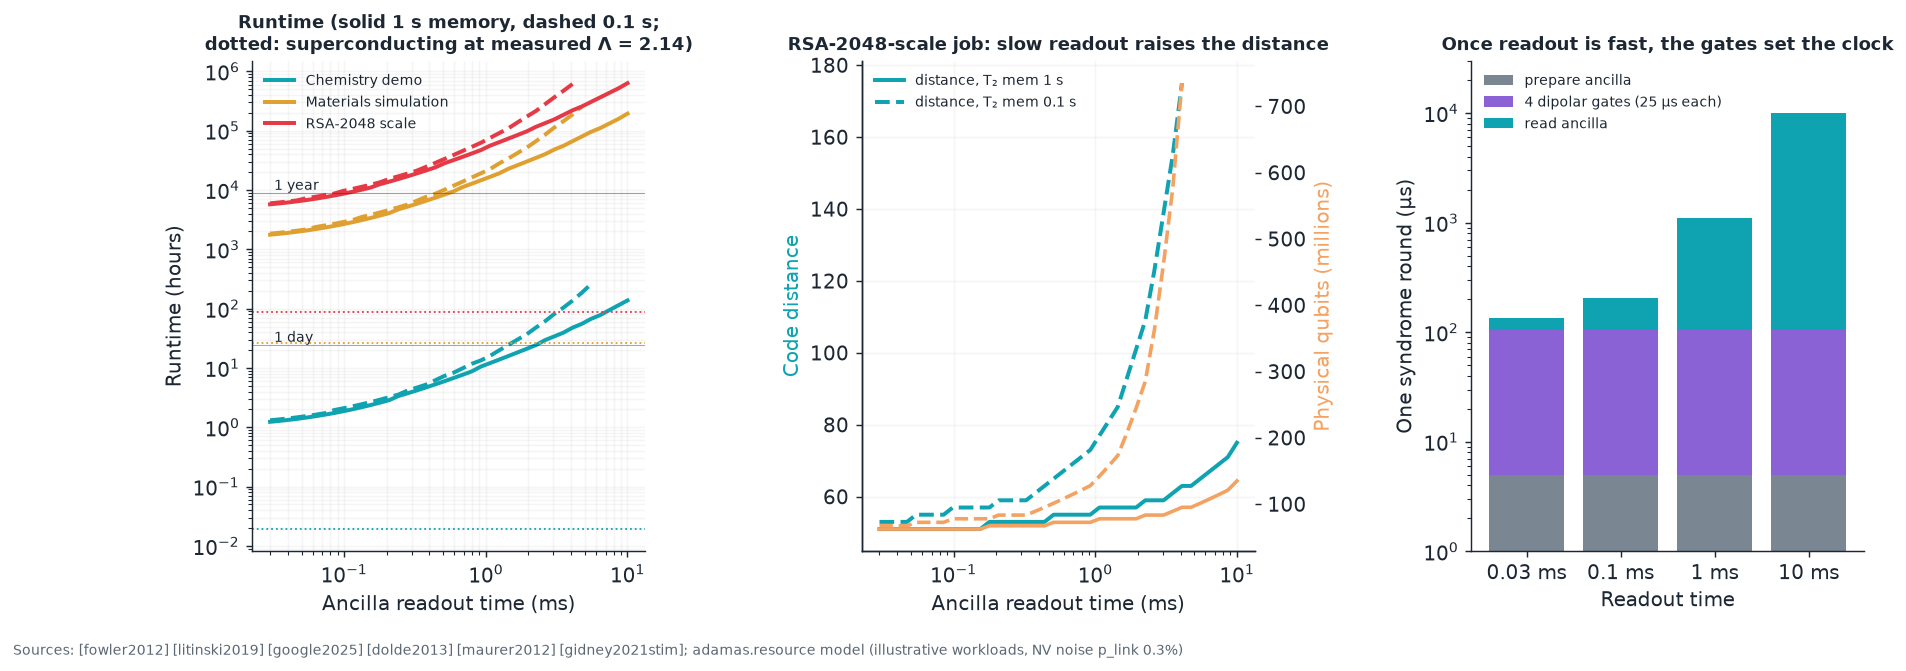
\includegraphics[width=\columnwidth]{fig39_resource_estimate.png}
\caption{Resource estimate from the circuit-level fits: runtime, code distance, and the composition of one syndrome round.}\label{fig:res}\end{figure}
Fitting $p_L(d)=A\Lambda^{-(d+1)/2}$ \cite{fowler2012} and pricing each logical step at $d$ rounds \cite{litinski2019} gives, for an RSA-2048-scale job (6{,}000 logical qubits, $3\times10^9$ steps), distance \RSADistance, \RSAQubitsM{} million physical qubits on a \RSADieMm\,mm die, and \RSAYears{} years at 1\,ms readout (\RSAYearsFast{} year at 0.1\,ms), against \RSADaysSC{} days for a superconducting machine at its measured $\Lambda=2.14$ \cite{google2025} (Fig.~\ref{fig:res}). If the gate noise is strongly biased (bias 100), the standard code needs distance \RSADistanceCSSBiased{} and \RSAQubitsMCSSBiased{} million qubits (\RSAYearsCSSBiased{} years), while a native XZZX code needs distance \RSADistanceXZZX{}, \RSAQubitsMXZZX{} million qubits, and \RSAYearsXZZX{} years: the bias of NV two-qubit gates decides which code to run. The NV figure assumes a 0.3\% link error that has not been demonstrated. Once readout is fast, the four dipolar gates dominate each round, so placement precision becomes the next lever.

\section{Experiments and teaching}
\begin{figure}[t]\centering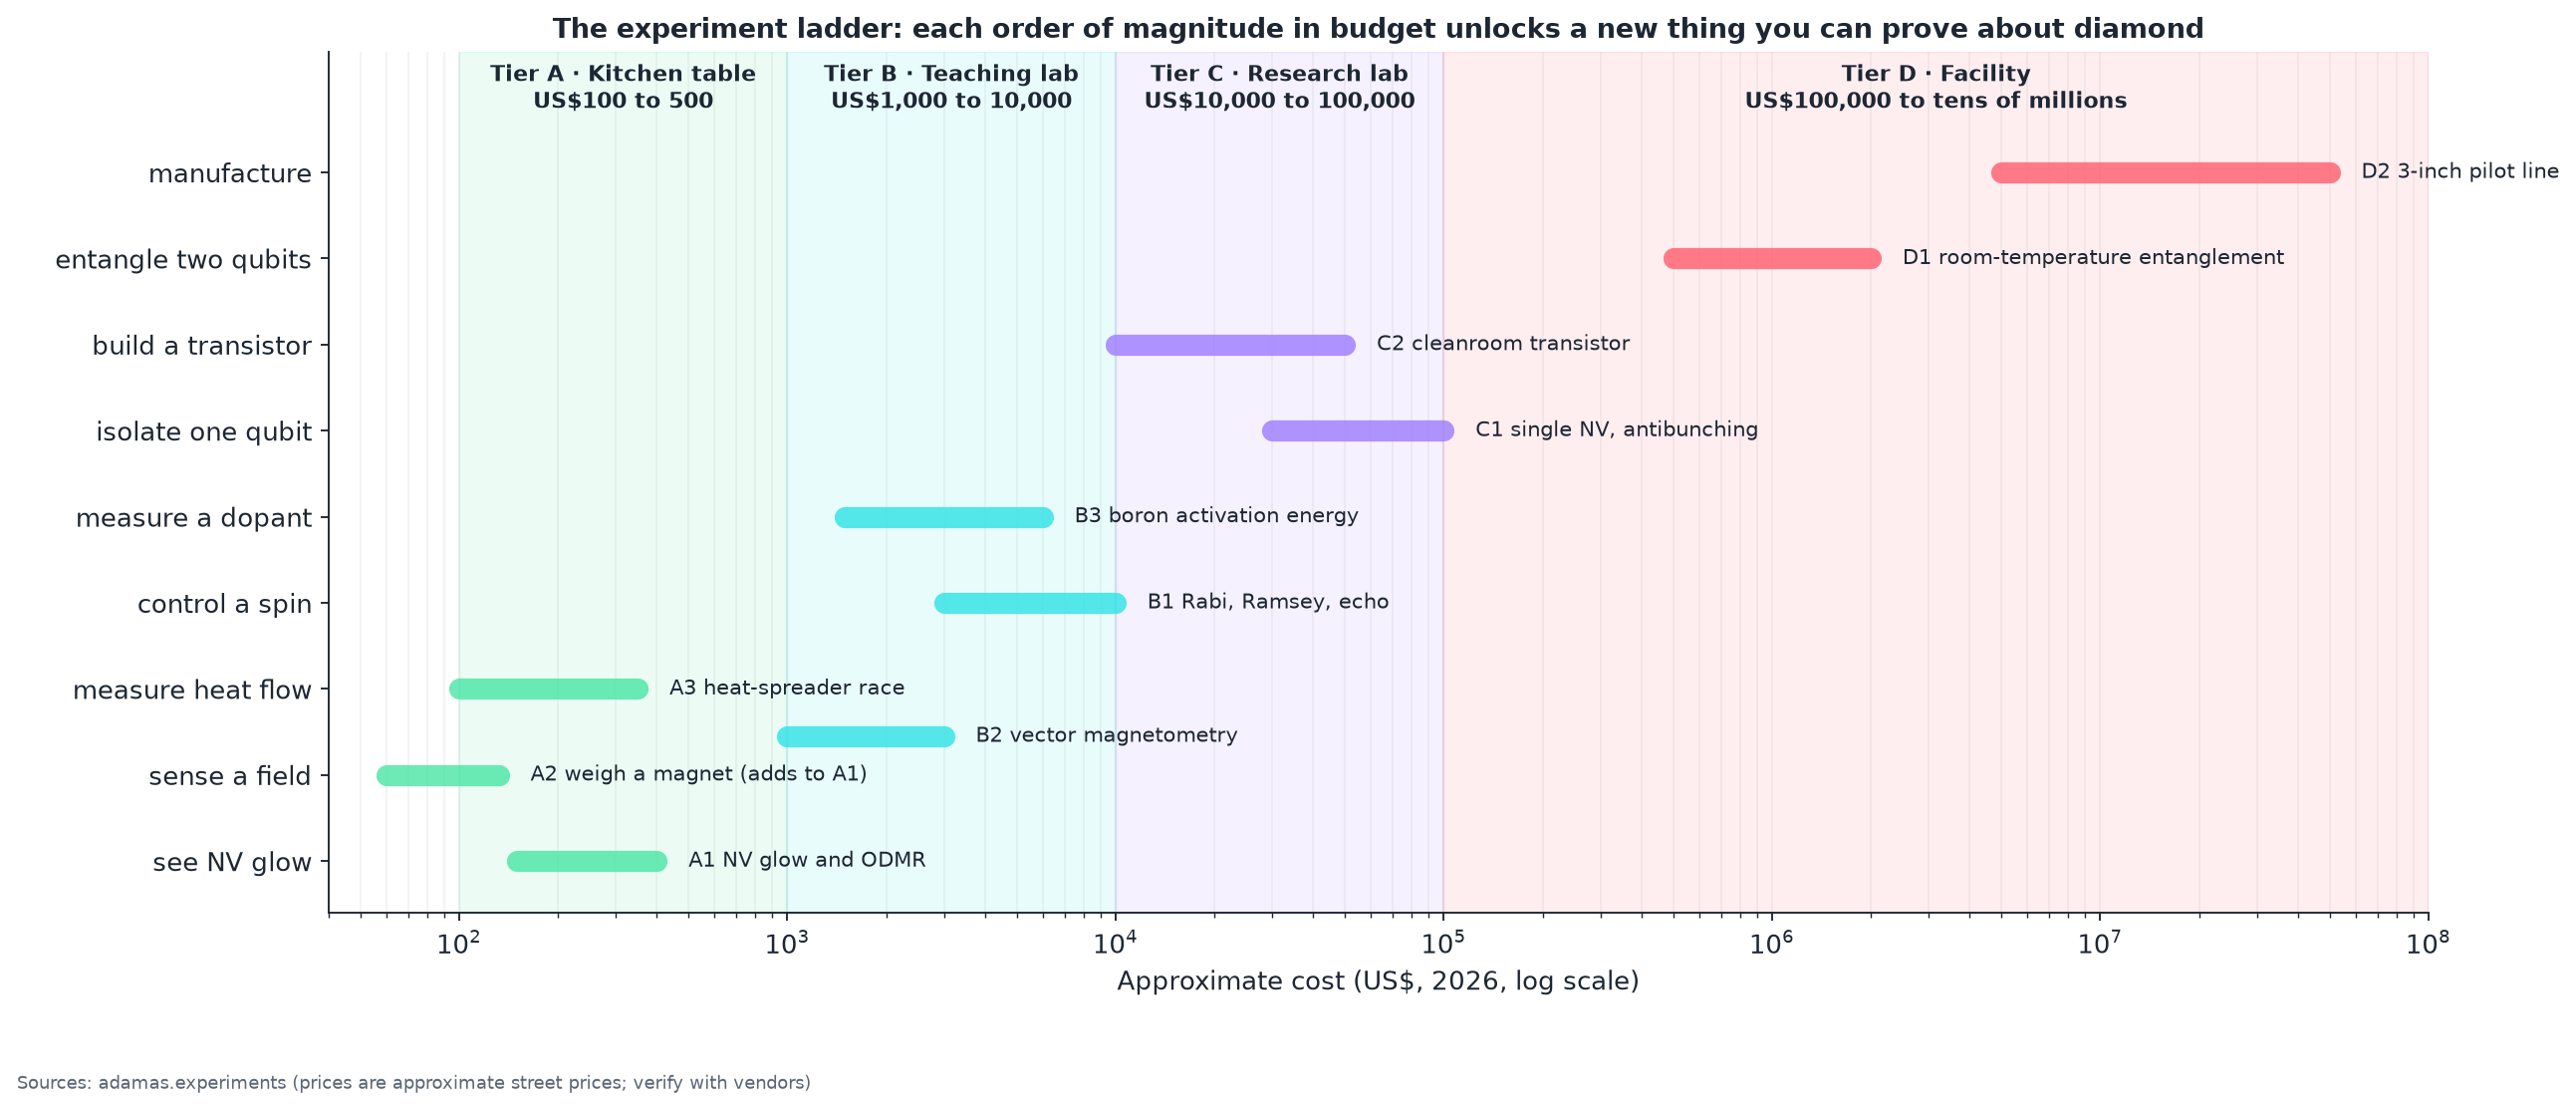
\includegraphics[width=\columnwidth]{fig47_experiment_ladder.png}
\caption{Ten experiments in four budgets, with parts, steps, safety, and simulated expected results; a firmware kit makes the US\$150 to 400 ODMR experiment runnable.}\label{fig:ladder}\end{figure}
Ten experiments span US\$100 to a pilot line (Fig.~\ref{fig:ladder}), following published teaching setups \cite{stegemann2023,williams2026,sewani2020}. The cheapest ships with firmware (Raspberry Pi Pico driving an ADF4351 synthesizer) and a host script whose output feeds the same fitting code as a browser Data Lab. A seven-lesson course, 13 interactive labs, and a process traveler turn the framework into teaching material; all browser simulations are tested against the Python models.

\section{Validation and uncertainty}
\begin{figure}[t]\centering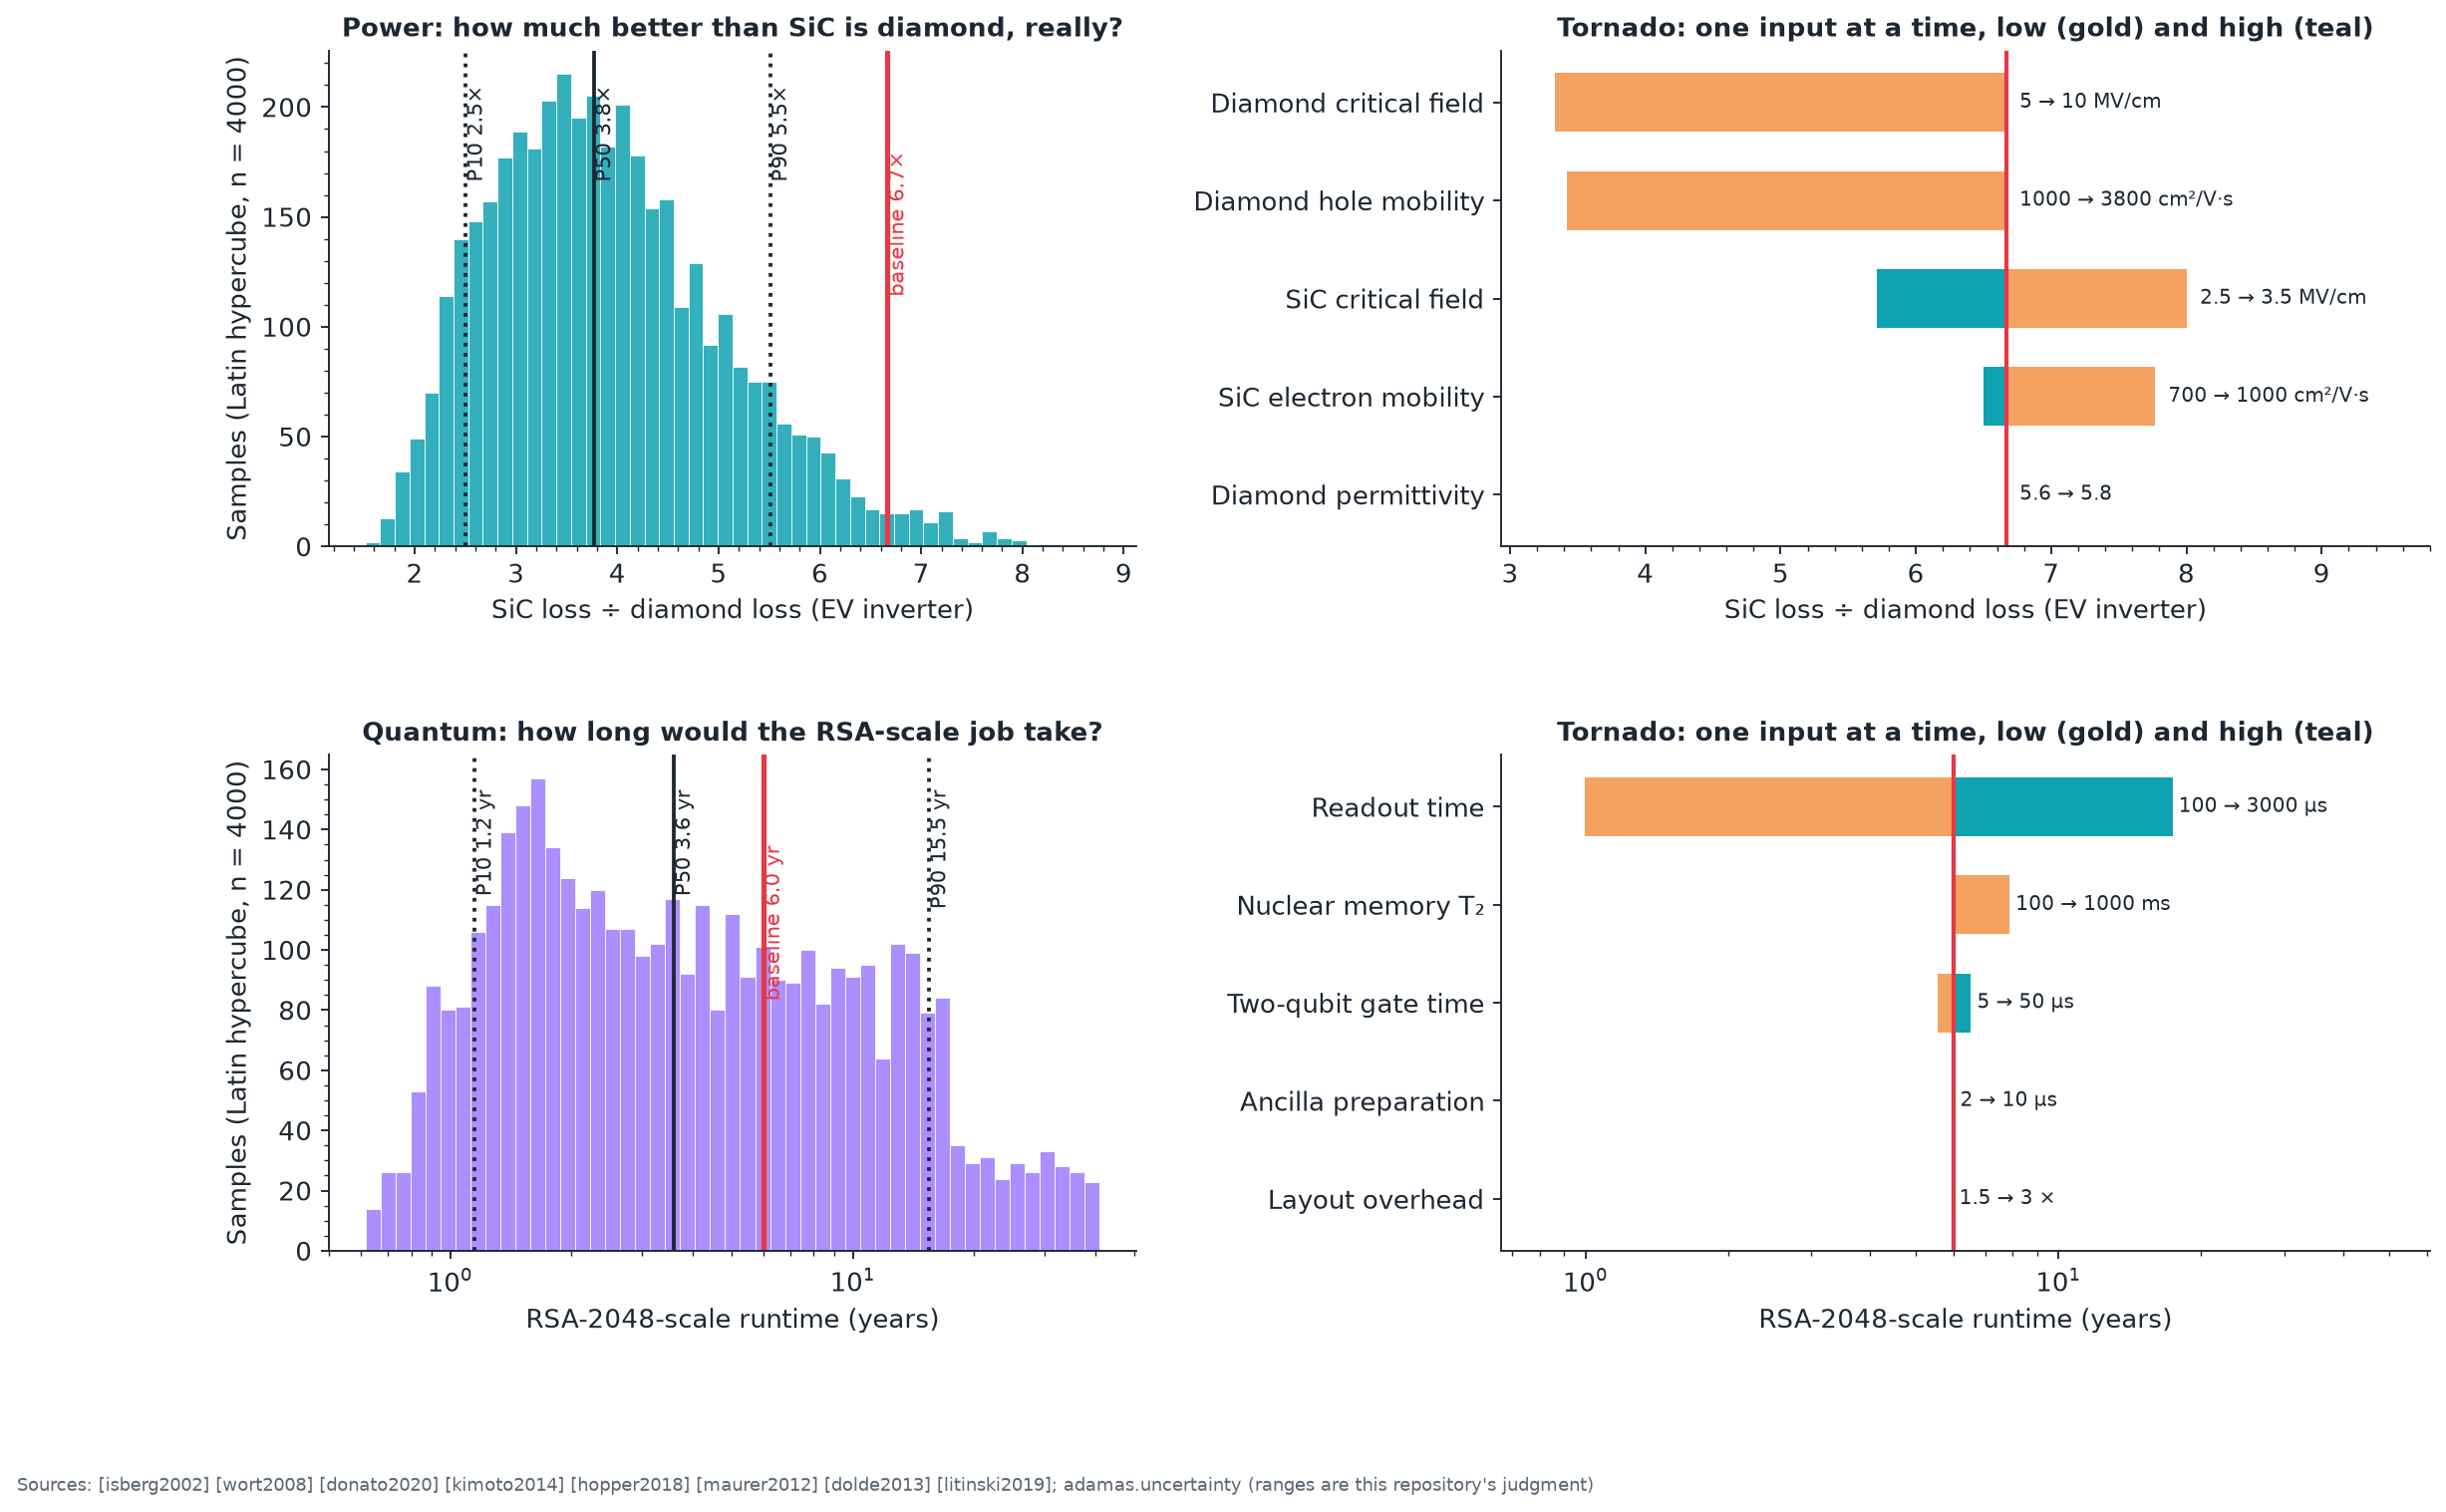
\includegraphics[width=\columnwidth]{fig49_uncertainty.png}
\caption{Latin-hypercube uncertainty propagation and tornado diagrams for the two headline results.}\label{fig:unc}\end{figure}
A validation matrix of \ValChecks{} checks (\ValPass{} pass, the rest explained discrepancies) compares each model with a published result, an independent tool, or a known answer; the phenomenological surface-code threshold, for example, reproduces the published 2.93\% to within 6\% \cite{wang2003}. Propagating the published spread of diamond's critical field and hole mobility \cite{isberg2002,wort2008,donato2020} lowers the silicon-carbide-to-diamond loss ratio from the optimistic baseline to a median of \UncPowerPfifty$\times$ (P10 to P90: \UncPowerPten{} to \UncPowerPninety$\times$). The runtime of the factoring-scale NV machine spans \UncQPten{} to \UncQPninety{} years (median \UncQPfifty), dominated by readout time (Fig.~\ref{fig:unc}).

\section{Limitations}
Transistor and switching parameters are literature-anchored placeholders until the PDK-0 monitor die is measured. The converter model omits gate charge and reverse recovery; the surface-code idle channel is phenomenological at the gate level (depolarizing or pure dephasing), and the native XZZX study assumes bias-preserving gate noise, which has not been measured for NV dipolar gates. Workloads in the resource estimate are illustrative scales.

\section*{Reproducibility}
\texttt{pip install -e ".[dev]" \&\& python -m pytest -q \&\& make figures paper} regenerates every figure, the numbers in this text (\texttt{python -m adamas.paper}), and this PDF. Interactive version: \site.

\small\bibliographystyle{unsrt}\bibliography{../references/references}
\end{document}
